\documentclass[11pt]{article}
\usepackage[utf8]{inputenc}
\usepackage[italian]{babel}
\usepackage{amssymb}
\usepackage{verbatim}
\usepackage{amsfonts}
\usepackage{amsmath}
\usepackage{multirow}
\usepackage{amsthm}
\usepackage{xcolor}
\usepackage{graphicx}
\usepackage{tikz}
\usepackage{float}
\usepackage[shortlabels]{enumitem}
\graphicspath{ {./images/} }
\usetikzlibrary{arrows}


\title{Titolo}
\author{Daniele De Micheli}
\date{2019}

\renewcommand*\contentsname{\textit{Indice}}

%presettaggio per teoremi e assiomi/definizioni%

\newtheorem*{nome}{teorema}

%fine%

\begin{document}

\maketitle
\tableofcontents

\part{Capitolo 1}
\section{Introduzione}
Questo documento è una sintesi degli appunti e dei concetti fondamentali necessari per poter affrontare con sicurezza l'esame di fisica nel nostro corso di studi. Come si può vedere dall'indice, il corso prevede tanti argomenti, che sono stati affrontati in modo non troppo approfondito e a volte forse in maniera superficiale. Spero di riuscire a creare una dispensa utile a chiunque voglia studiare senza dover comprare un libro e magari anche per chi per voglia o necessità non può seguire il corso fisicamente.
\subsection{Grandezze fondamentali e derivate}
Le \textit{grandezze fondamentali} e le \textit{grandezze derivate} sono \textbf{grandezze fisiche}, ossia caratteristiche di un corpo o di uno stato di un fenomeno che può essere misurata tramite strumenti ed esperimenti ed espressa tramite numeri e unità di misura.

Possiamo distinguere le due grandezze come segue:
\begin{itemize}
	\item Grandezze fondamentali: sono grandezze indipensdenti, cioè che non vengono definite a partire da altre grandezze. Alcuni esempi di grandezze fondamentali sono:
	\begin{itemize}
		\item Lunghezza: generalmente indicata con il simbolo L, è definita tramite il \textit{metro}, il quale è calcolato come la distanza che percorre la luce (nel vuoto), in un tempo di $\dfrac{1}{299729458}$ secondi.
		\item Tempo: si indica con la lettera T e rappresenta un concetto astratto. La sua unità di misura è il \textit{secondo} ed è calcolato come la durata di un determinato numero di oscillazioni complete di un atomo di Cesio 133.
		\item Massa: viene indicata dalla lettera M, la sua unità di misura è il \textit{chilogrammo} ed è definito tramite una proprietà fisica correlata ad una costante fondamentale, ossia come la quantità di massa per compensare una forza di $6,626 070 15 * 10^34$ J al s. 
		\item Temperatura: questa grandezza è rappresentata dalla lettera greca $\Theta$ e si misura in \textit{kelvin}.  Lo 0 kelvin è definito come \textit{zero assoluto}; il kelvin è inoltre definito come $\frac{1}{273,16}$ della temperatura del \textbf{punto triplo dell'acqua}.
	\end{itemize}
	\item Intensità di corrente: si indica con la lettera I, la sua unità di misura è l'\textit{ampere}. L'ampere è definito in maniera fisica come la forza di uno spostamento.
	\item Quantità di materia: viene indicata con la lettera N e si misura in \textit{mole}. Una mole corrisponde alla quantità di materia che contiene tante entità elementari quanti sono gli atomi presenti in 12 grammi di carbonio 12.
	\item Grandezze derivate: sono grandezze che nascono dalle grandezze fondamentali. Alcuni esempi di grandezze derivate che useremo sono:
	\begin{itemize}
		\item Volume: è una grandezza derivata definita come la misura nello spazio occupato da un solido.
		\item Velocità: è la quantità di spazio percorso rispetto ad una unità di tempo predefinita.
		\item Densità: rappresenta la quantità di massa in un'unità di volume.
	\end{itemize}
\end{itemize}

\subsection{Grandezze Scalari e Vettoriali}
Di grandezze ne esisitono di due tipi distinti, grandezze \textit{scalari} e grandezze \textit{vettoeiali}. Le prima sono rappresentabili tramite un semplice numero scalare, che rappresenta direttamente la "quantità" della grandezza. Per esempio, la temperatura è una grandezza scalare, come anche la massa.

Le grandezze vettoriali invece, possiedono delle caratteristiche oltre alla sola "quantità" di grandezza. Le proprietà sono 3:
\begin{itemize}
	\item \textbf{Modulo}: il modulo è la grandezza scalare della misura. Si potrebbe dire che è l'unica proprietà che possiedono le grandezze scalari.
	\item \textbf{Direzione}: rappresenta la direzione della grandezza. Di solito la direzione viene rappresentata tramite un segmento direzionato che giace su di una retta la quale indica la direzione del vettore.
	\item \textbf{Verso}: il verso rappresenta il "segno" della direzione; data un'origine è possibile capire rispetto ad essa se la grandezza è positiva o negativa.
\end{itemize}
Alcuni esempi di grandezze vettoriali sono la \textit{velocità} $\overrightarrow{v}$, l'accelerazione $\overrightarrow{a}$ o ancora la forza $\overrightarrow{F} = m*\overrightarrow{a}$, che è il prodotto di una grandezza scalare per una vettoriale.
\paragraph{Sistema di riferimento} Per poter utilizzare in modo corretto i vettori e le grandezze vettoriali, abbiamo bisogno di introdurre il concetto di \textit{\textbf{Sistema di riferimento}}: questo può essere visto come un'insieme di assi cartesiani che rappresentano lo spazio (monodimensionale, bidimensionale o tridimensionale). Generalmente utilizzeremo questi tre sistemi per rappresentare il mondo fisico che ci circonda.


Nello studiare un fenomeno, la scelta del sistema di riferimento è indipendente dallo spostamento.
\section{Cinematica}
\subsection{Velocità media e istantanea}
Prima di definire queste due grandezze, iniziamo con il definire i concetti di \color{red} distanza \color{black} e \color{red} spostamento\color{black}.
\\ \\
La \textit{distanza} è la quantità di spazio percorso in totale.
\\ \\
Lo \textit{spostamento} rappresenta, rispetto all'origine, di quando mi sono spostato. Potremmo vederla come una distanza relativa all'origine.

\begin{figure}[H]
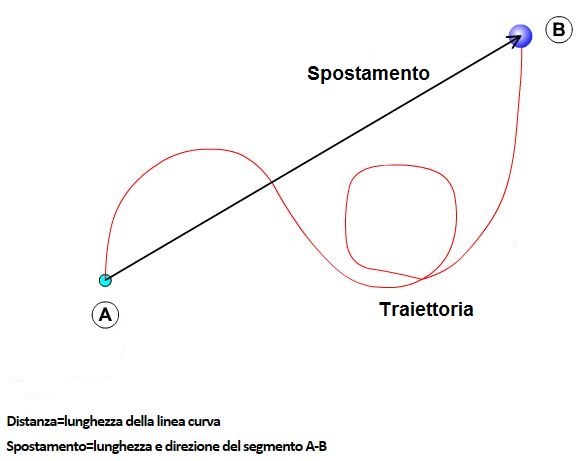
\includegraphics[scale=0.5]{distanza_spostamento.jpg}
\centering
\end{figure}

\section{Dinamica}
\section{Lavoro ed Energia}

Prendiamo un piano su cui poniamo una molla e un oggetto che si muove con velocità $v$ e con massa $m$.



\section{Gravitazione}
\part{Capitolo 2}
\section{Fluidodinamica}

\section{Termodinamica}

\section{Elettrostatica e Elettrotecnica}

\section{Magnetismo}




\end{document}
